\subsection{Introduction}

The ILC accelerator is planned with one interaction region, equipped
with two experiments. The two experiments are swapped into the
Interaction Point within the so-called "Push-Pull" scheme. The
experiments have been designed to allow fast move-in and move-out from
the interaction region, on a timescale of a few hours to a day. In
2008 a call for letters of intent was issued to the
community. Following a detailed review by an international detector
advisory group, two experiments were selected in 2009 and invited to
prepare more detailed proposals.  These  are the SiD detector and the ILD
detector described in this section. Both prepared detailed and costed proposals which were
scrutinised by the international advisory group and included in the
2012 ILC
Technical Design Report~\cite{Behnke:2013lya}.  In this section the two proposals are
briefly   introduced.

The ILC detectors are designed to make precision measurements on the
Higgs boson,  $W$, $Z$, $t$, and other particles.    They are able to
meet the requirements for such measurements, first, because the
experimental conditions are naturally very much more benign than those
at the LHC, and second, because the detector collaborations have
developed technologies specifically to take advantage of these more
forgiving conditions. 

An $\ee$ collider gives much  lower collision
rates and events of much lower complexity than a hadron collider, 
and detectors can be adapted to take
advantage of this.  The radiation levels at the ILC will be modest compared with the
LHC, except for the special forward calorimters very close to the
beamline, where radiation exposure will be an issue. 
This  allows the consideration of a wide range of
materials and technologies for the tracking and calorimeter systems. 
The generally low
radiation levels allow the innermost vertex detector elements to
be located at very small  radii, significantly enhancing the efficiency
for short-lived particle identification. More generally,  the relatively
benign ILC experiment environment permits  the design of 
tracking detectors with minimal material profile (see
Sec.~\ref{sub:sw-sim}).  This allows the detectors to meet the
stringent requirement on the track momentum resolution
 which is driven by the needs to reconstruct sufficiently precisely
 the Z-mass in the Higgs recoil analysis.  This requirement translates into a system
 resolution nearly an order of magnitude better than achieved in the
 LHC experiments.

At the same time, although they are studying electroweak particle
production, it is essential that the ILC detectors have excellent
performance for jets.   At an $\ee$ collider, $W$ and $Z$ bosons are
readily observed in their hadronic decay modes, and the study of these
modes plays a major role in most analyses.    To meet the requirements
of precision measurements, the ILC detectors are optimized from the
beginning to enable jet reconstruction and measurement using 
the particle-flow algorithm (PFA). This drives the goal of $3\%$
 jet mass resolution at energies above 100~\GeV,  a resolution
about twice as good as has been achieved in  the LHC
 experiments.

FInally, while the LHC detectors depend crucially on multi-level
triggers that filter out only a small fraction of events for analysis,
the  rate of interactions at the ILC is sufficiently low to allow
running without a trigger.     The ILC accelerator design is based on
trains of electron and positron bunches, with a repetition rate of
5~Hz, and with 1312 bunches (and bunch
collisions) per train (see Sec.~\ref{sec:ilc},
Tab.~\ref{tab:ilc-params}). 
The 199 ms interval between bunch trains provides ample time for a full
readout of data
 from the  previous train.  While there are background processes arising
 from  beam-beam interactions, the detector occupancies arising from these 
have been shown to be manageable.

The combination of extremely precise tracking, excellent jet mass
resolution, and triggerless running gives the ILC, at 250 GeV and at
higher energies, a superb potential for discovery. 

To meet these goals an ambitious R\& D program has
 been pursued throughout the past 10 years or so to develop and
 demonstrate the needed technologies. The results of this program are
 described in some detail in Ref.~\cite{RDliaision}. 
 The two experiments proposed for
 the ILC, SiD and ILD, utilise and 
rely on the results from these R\&D efforts.

Since the goals of SiD and ILD in terms of material budget, tracking
performance, heavy-flavor tagging, and jet mass resolution are very 
demanding, we feel it important to provide information about the level
of detailed input that enters our performance estimates.   These are
best
discussed together with the event reconstruction and analysis
framework that we will present in Sec.~\ref{sec:software}.   In that
section, we will present estimates of detector performance as
illustrations at the successive stages of event analysis. 



\subsection{The SiD Detector}
The SiD detector is a general-purpose experiment designed to perform
 precision measurements
at the ILC. It satisfies the challenging detector requirements resulting from the full range of 
ILC physics processes. SiD is based on the paradigm of particle flow, an algorithm by which
the reconstruction of both charged and neutral particles is accomplished by an optimised
combination of tracking and calorimetry. The net result is a significantly more precise jet
energy measurement which results in a di-jet mass resolution good enough to distinguish
between $W$s and $Z$s.
The SiD detector (Fig.~\ref{fig:fig_sid})  is a compact detector based on a powerful silicon
pixel vertex detector, silicon tracking, silicon-tungsten electromagnetic calorimetry, and
highly segmented hadronic calorimetry. 
SiD also incorporates a high-field solenoid, iron
flux return, and a muon identification system. The use of silicon 
sensors in the vertex, tracking,
and calorimetry enables a unique integrated tracking system ideally suited to particle
flow.

The choice of silicon detectors for tracking and vertexing ensures that SiD is robust
with respect to beam backgrounds or beam loss, provides superior charged particle momentum
resolution, and eliminates out-of-time tracks and backgrounds. The main tracking
detector and calorimeters are “live” only during a single bunch crossing, so beam-related
backgrounds and low-pT backgrounds from $\gamma\gamma$ processes will be reduced to the minimum
possible levels. The SiD calorimetry is optimised for excellent jet energy measurement
using the particle flow technique.
 The complete tracking and calorimeter systems are contained
within a superconducting solenoid, which has a 5 T field strength, enabling the overall
compact design. The coil is located within a layered iron structure
that returns the magnetic flux and is instrumented to allow the
identification of muons. 
All aspects of SiD are the result of intensive and leading-edge research aimed at achieving
performance at unprecedented levels. At the same time, the design represents a balance between cost
and physics performance. The key parameters of the SiD design are
listed in  
Table~\ref{sid:ConceptOverview:Table:Ovw_sidparams}.

\begin{figure}[tb]
 %\epsfysize=9.0cm
 \begin{center}
 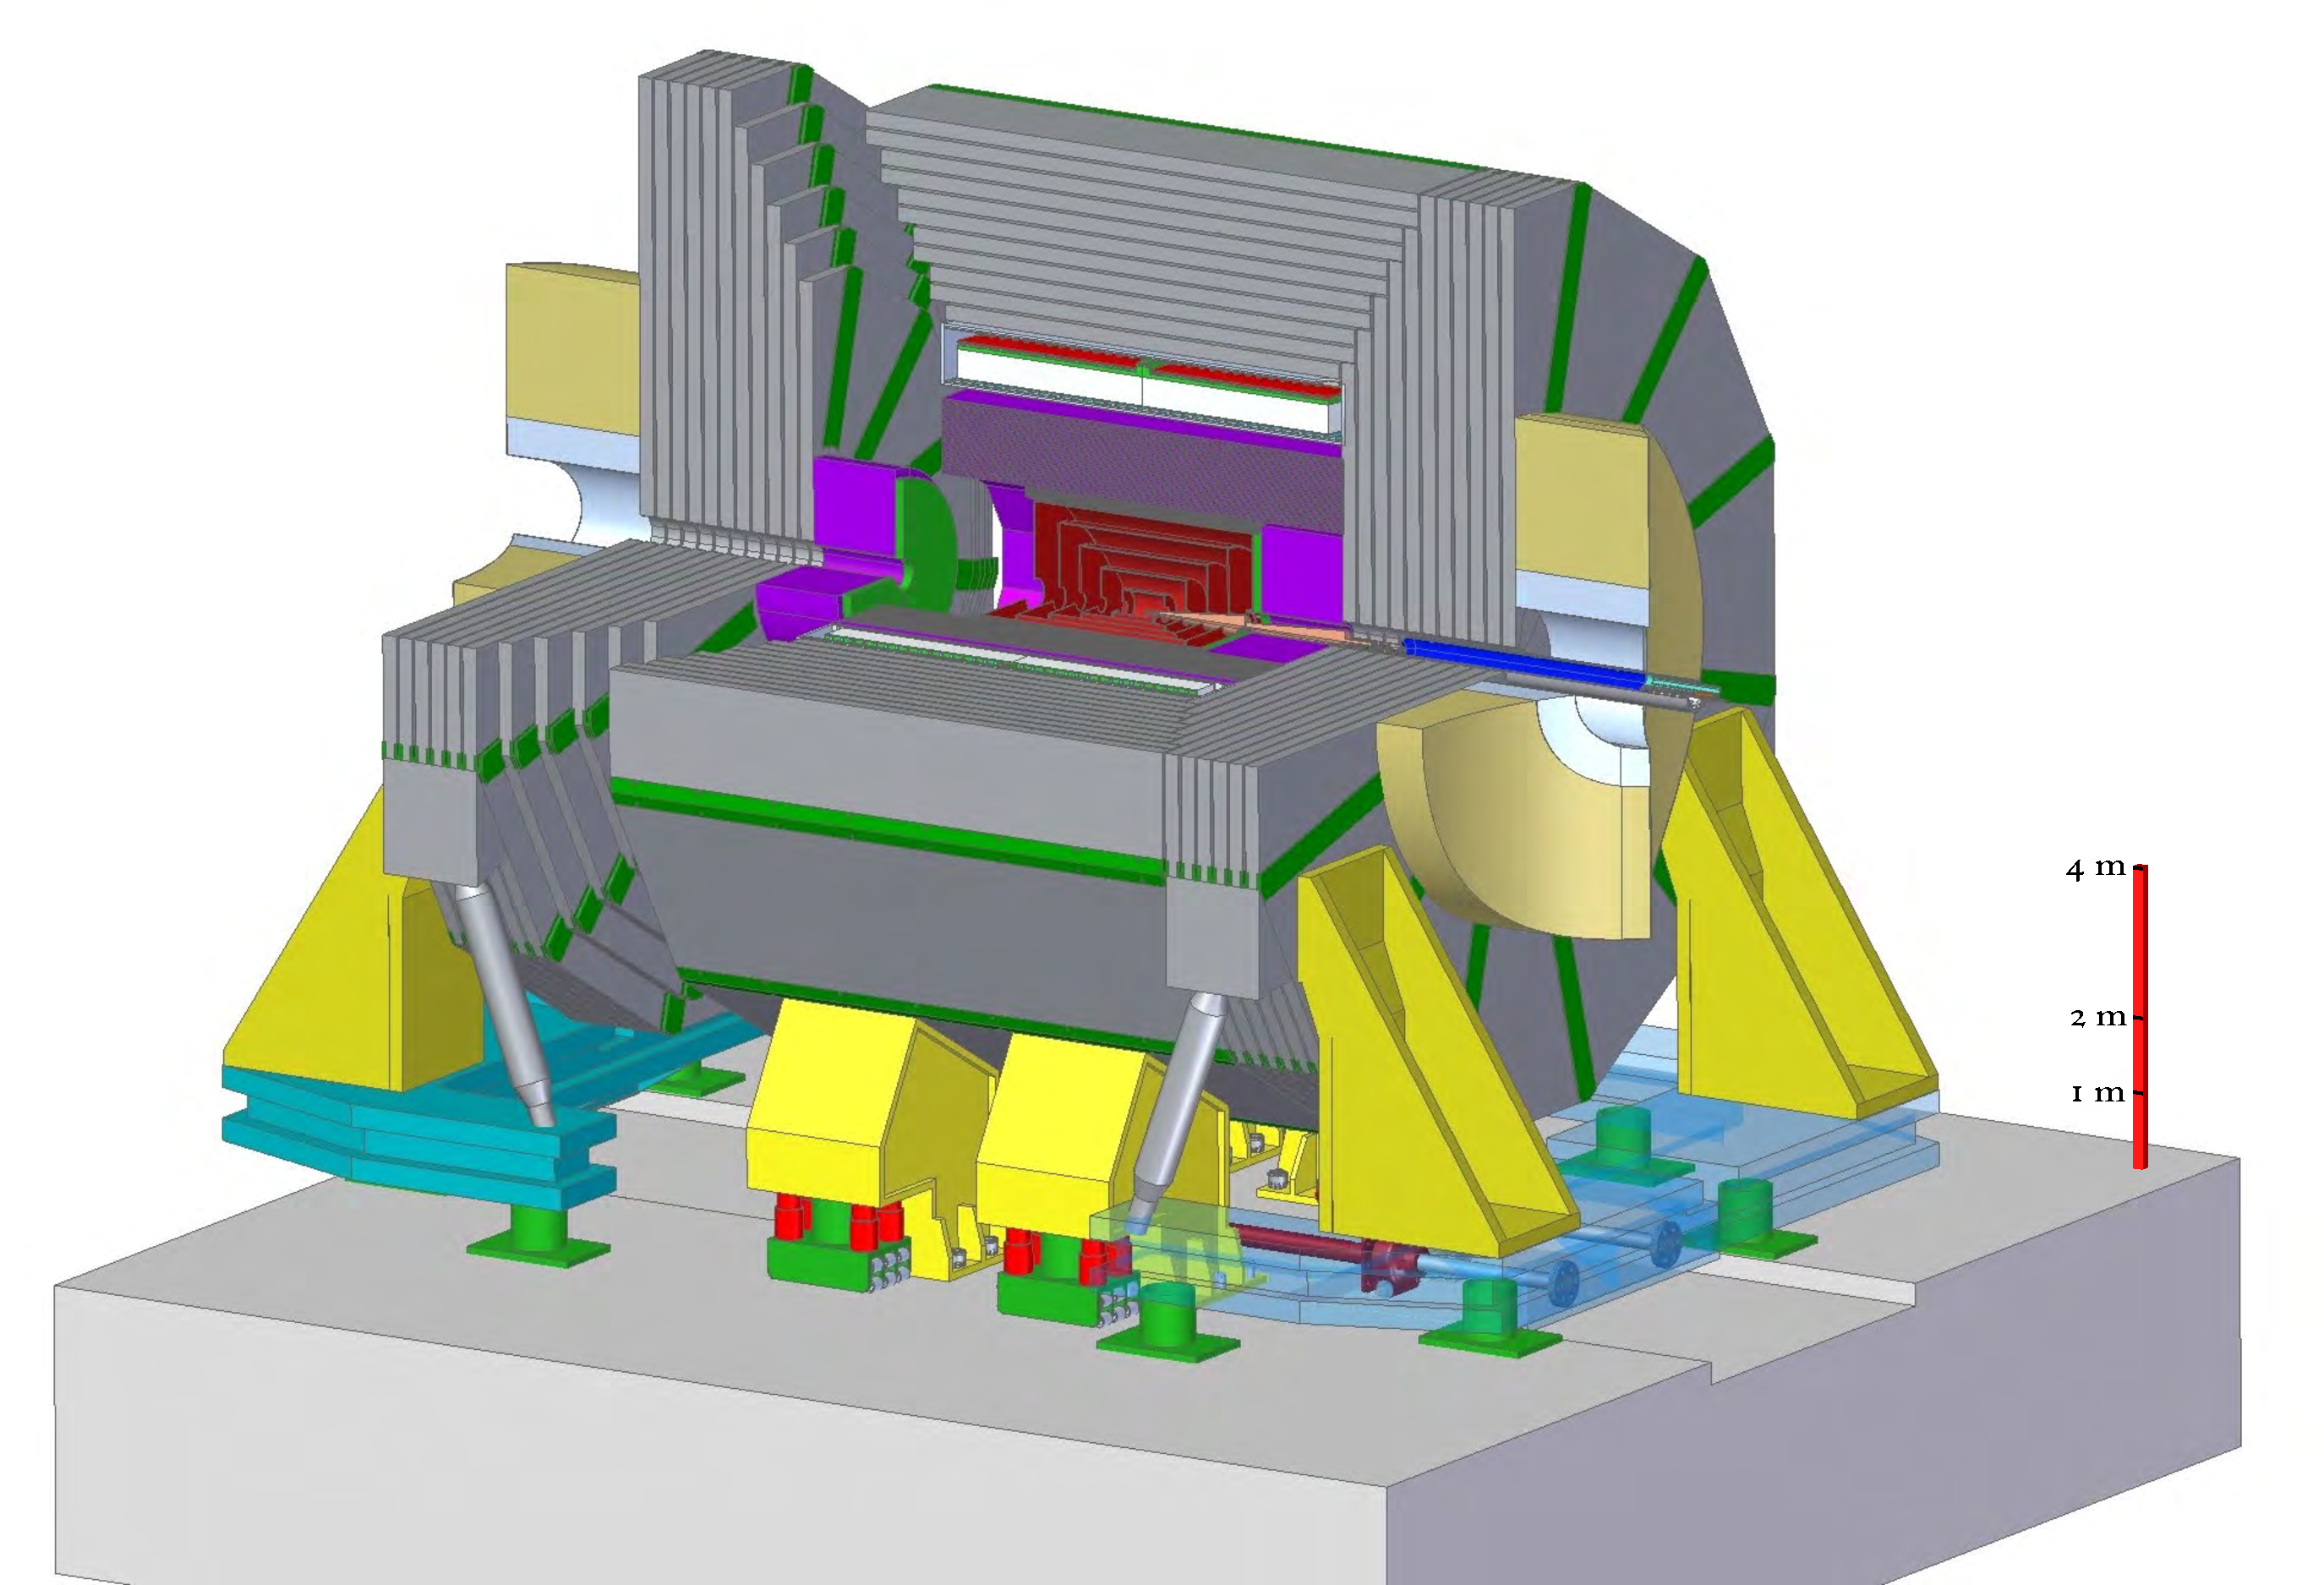
\includegraphics[width=0.9\hsize]{chapters/figures/SiD.pdf}
\caption{The SiD detector concept.
\label{fig:fig_sid}}
 \end{center}
 \vspace{-0.7cm}
 \end{figure}

%\thisfloatsetup{floatwidth=\SfigwFull,capposition=beside}
\begin{table}[htbp]
\renewcommand{\arraystretch}{1.25}

%fixme: ttabbox is not known ...
%\ttabbox{

\caption{\label{sid:ConceptOverview:Table:Ovw_sidparams}Key parameters of the baseline \sid design. (All dimension
are given in cm).}

{
\begin{tabular}{l l r r r}
    \toprule
    \sid Barrel& Technology& In rad& Out rad& z extent \\
    \midrule
    Vtx detector& Silicon pixels& 1.4& 6.0& $\pm \quad 6.25$ \\
    Tracker& Silicon strips& 21.7& 122.1& $\pm \quad 152.2$ \\
    ECAL& Silicon pixels-W& 126.5& 140.9& $\pm \quad 176.5$ \\
    HCAL& RPC-steel& 141.7& 249.3& $\pm \quad 301.8$ \\
    Solenoid& 5 Tesla SC & 259.1& 339.2& $\pm \quad 298.3$ \\
    Flux return& Scint-steel& 340.2 & 604.2& $\pm \quad 303.3$ \\
    \bottomrule

   \toprule
 \sid Endcap& Technology& In z& Out z& Out rad \\
    \midrule
Vtx detector& Silicon pixels& 7.3& 83.4& 16.6 \\
Tracker& Silicon strips& 77.0& 164.3& 125.5 \\
ECAL& Silicon pixel-W& 165.7& 180.0& 125.0 \\
HCAL& RPC-steel& 180.5& 302.8& 140.2 \\
Flux return& Scint/steel& 303.3& 567.3& 604.2 \\
LumiCal& Silicon-W& 155.7& 170.0& 20.0 \\
BeamCal& Semicond-W& 277.5& 300.7& 13.5 \\
    \bottomrule
\end{tabular}
}

\end{table}

\subsubsection{Silicon-based Tracking}
The tracking system (Fig.~\ref{fig:fig_vxdtrk}) is a key element of the SiD detector concept. The
particle flow algorithm requires excellent tracking with superb efficiency and
two-particle separation. The requirements for precision measurements, in
particular in the Higgs sector, place high demands on the momentum resolution at
the level of $\delta (1/\pT)  \sim 2-5 \times 10^{-5}/$GeV/$c$.

Highly efficient charged particle tracking is achieved using the pixel detector
and main tracker to recognise and measure prompt tracks, in conjunction with the ECAL, which can
identify short track stubs in its first few layers 
to catch tracks arising from secondary decays of long-lived particles. With
the choice of a 5~T solenoidal magnetic field, in part chosen to control the $\ee$-pair
background, the design allows for a compact tracker design. 

\begin{figure}[tb]
 %\epsfysize=9.0cm
 \begin{center}
 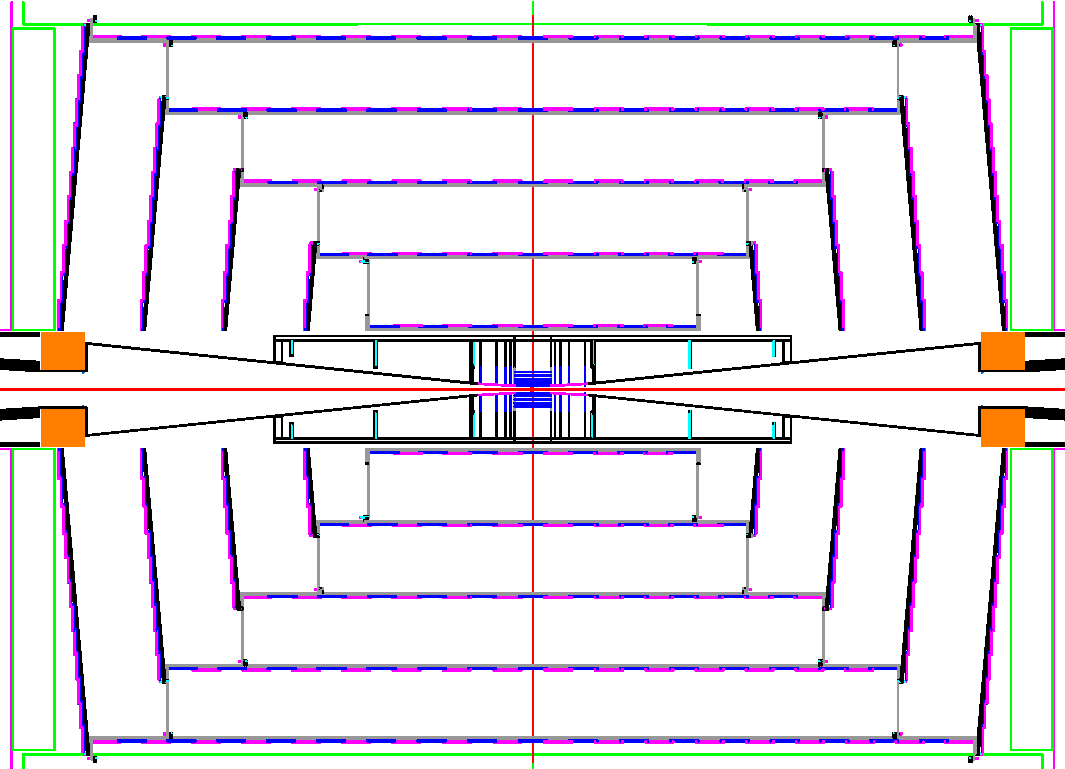
\includegraphics[width=0.9\hsize]{chapters/figures/vxdtrk.pdf}
\caption{r-z view of vertex detector and outer tracker.
\label{fig:fig_vxdtrk}}
 \end{center}
 \vspace{-0.7cm}
 \end{figure}

\subsubsection{Vertex detector}

To unravel the underlying physics mechanisms of new observed processes, the
identification of heavy flavours will play a critical role. One of the main
tools for heavy flavour identification is the vertex detector. The physics goals
dictate an unprecedented spatial three-dimensional point resolution and a very
low material budget to minimise multiple Coulomb scattering. The running 
conditions at the ILC impose the readout speed and radiation tolerance. 
These requirements are normally in tension. High
granularity and fast readout compete with each other and tend to increase the
power dissipation. Increased power dissipation in turn leads to an increased
material budget. The challenges on the vertex detector are considerable and
significant R\&D is being carried out on both the development of the sensors and
the mechanical support.
The SiD vertex detector uses a barrel and disk layout. The barrel section
consists of five silicon pixel layers with a pixel size of
$20~\times~20~\micron^2$. The forward and backward regions each have four
silicon pixel disks. In addition, there are three silicon pixel disks at a
larger distance from the interaction point to provide uniform coverage for the
transition region between the vertex detector and the outer tracker. This
configuration provides for very good hermeticity with uniform coverage and
guarantees excellent charged-track pattern recognition capability
 and impact parameter resolution 
over the full solid angle. 
This enhances the capability of the integrated tracking system and, 
in conjunction with the high magnetic field, makes for a very compact
system, thereby minimising the size and costs of the calorimetry.

To provide for a very robust track-finding performance the baseline 
choice for the vertex detector has a sensor technology that provides
time-stamping of each hit with sufficient precision to assign it to
a particular bunch crossing. This significantly suppresses
backgrounds. 

%Several technologies are being developed. One of them is a CMOS-based
%monolithic pixel sensor called Chronopixel. The main goal for the design is a
%pixel size of about $10~\times~10~\micron^2$ with 99\% charged-particle
% efficiency. Prototype devices have demonstrated that the concept works; 
%what should be a fully functional chip is presently under test. More 
%challenging is the 3D vertical integrated silicon technology, for which a full 
%demonstration is also close.

Several vertex detector sensor technologies are being developed.  One of these is a 
monolithic CMOS pixel detector with time-stamping capability (Chronopixel~\cite{Sinev:2015iwr}),
being developed in collaboration with SRI International. 
The pixel size is about  $10~\times~10~\micron^2$ with a design goal of 99\% charged-particle
 efficiency.
The time-stamping feature of the design means each hit is accompanied by a time tag with sufficient precision to assign it to a particular bunch crossing of
the ILC -- thus the name Chronopixel. This reduces the occupancy to negligible levels, even in the
innermost vertex detector layer, yielding a robust vertex detector which operates at background
levels significantly in excess of those currently foreseen for the ILC. Chronopixel differs from the
similar detectors developed by other groups by its capability to record time stamps for two hits in
each pixel while using standard CMOS processing for manufacturing. 
Following a series of prototypes, the Chronopixel has been proven to be
a feasible concept for the ILC. The three prototype versions
were fabricated in 2008, in 2012, and in 2014.
The main goal of the third prototype was to test possible solutions for a high capacitance problem
discovered in prototype 2. The problem was traced to the TSMC 90 nm technology design rules,
which led to an unacceptably large value of the sensor diode capacitance. Six different layouts
for the prototype 3 sensor diode were tested, and the tests demonstrated that the high capacitance
problem was solved.

With prototype 3 proving that a Chronopixel sensor can be successful with all known problems solved, optimal sensor design would be the focus of future tests.
The charge collection efficiency for different sensor diode options needs to be measured to determine
the option with the best signal-to-noise ratio. Also, sensor efficiency for charged particles with sufficient energy to penetrate the sensor thickness and ceramic package, along with a trigger telescope measurement, needs to be determined. Beyond these fundamental measurements, a prototype of a few cm$^2$ with a final readout scheme would
test the longer trace readout resistance, capacitance, and crosstalk.

A more challenging approach is the 3D vertical integrated silicon technology, for which a full 
demonstration is also close.




Minimising the support material is critical to the development of a high-performance 
vertex detector. An array of 
low-mass materials such as reticulated foams and silicon-carbide
materials are under consideration. An alternative approach that is being pursued very actively is the
embedding of thinned, active sensors in ultra low-mass media. This line of R\&D
explores thinning active silicon devices to such a thickness that the silicon
becomes flexible. The devices can then be embedded in, for example, Kapton
structures, providing extreme versatility in designing and constructing a vertex
detector.

Power delivery must be accomplished without exceeding the material budget and
overheating the detector.  The vertex detector 
design relies on power pulsing during bunch trains to minimise heating 
and uses forced air for cooling. 

\subsubsection{Main tracker}
The main tracker technology of
choice is silicon strip sensors arrayed in five nested cylinders in the central
region and four disks following a conical surface with an angle of 5 degrees
with respect to the normal to the beamline in each of the end regions. The geometry of the endcaps
minimises the material budget to enhance forward tracking. The detectors are
single-sided silicon sensors, approximately 10 $\times$ 10 cm$^2$ with a readout
pitch of 50~\micron. The endcaps utilise two sensors bonded back-to-back for
small angle stereo measurements. With an outer cylinder radius of 1.25~m
and a 5~T field, the charged track momentum resolution will be better than
$\delta (1/\pT) = 5 \times 10^{-5} $/(GeV/$c$) for high momentum tracks with coverage down to polar angles of 10 degrees.
A plot of the momentum budget as a function of polar angle is shown in Fig.~\ref{fig:sid_mat_budget}.

%%%%%%%%%%%%%%%%
\begin{figure}
\begin{center}
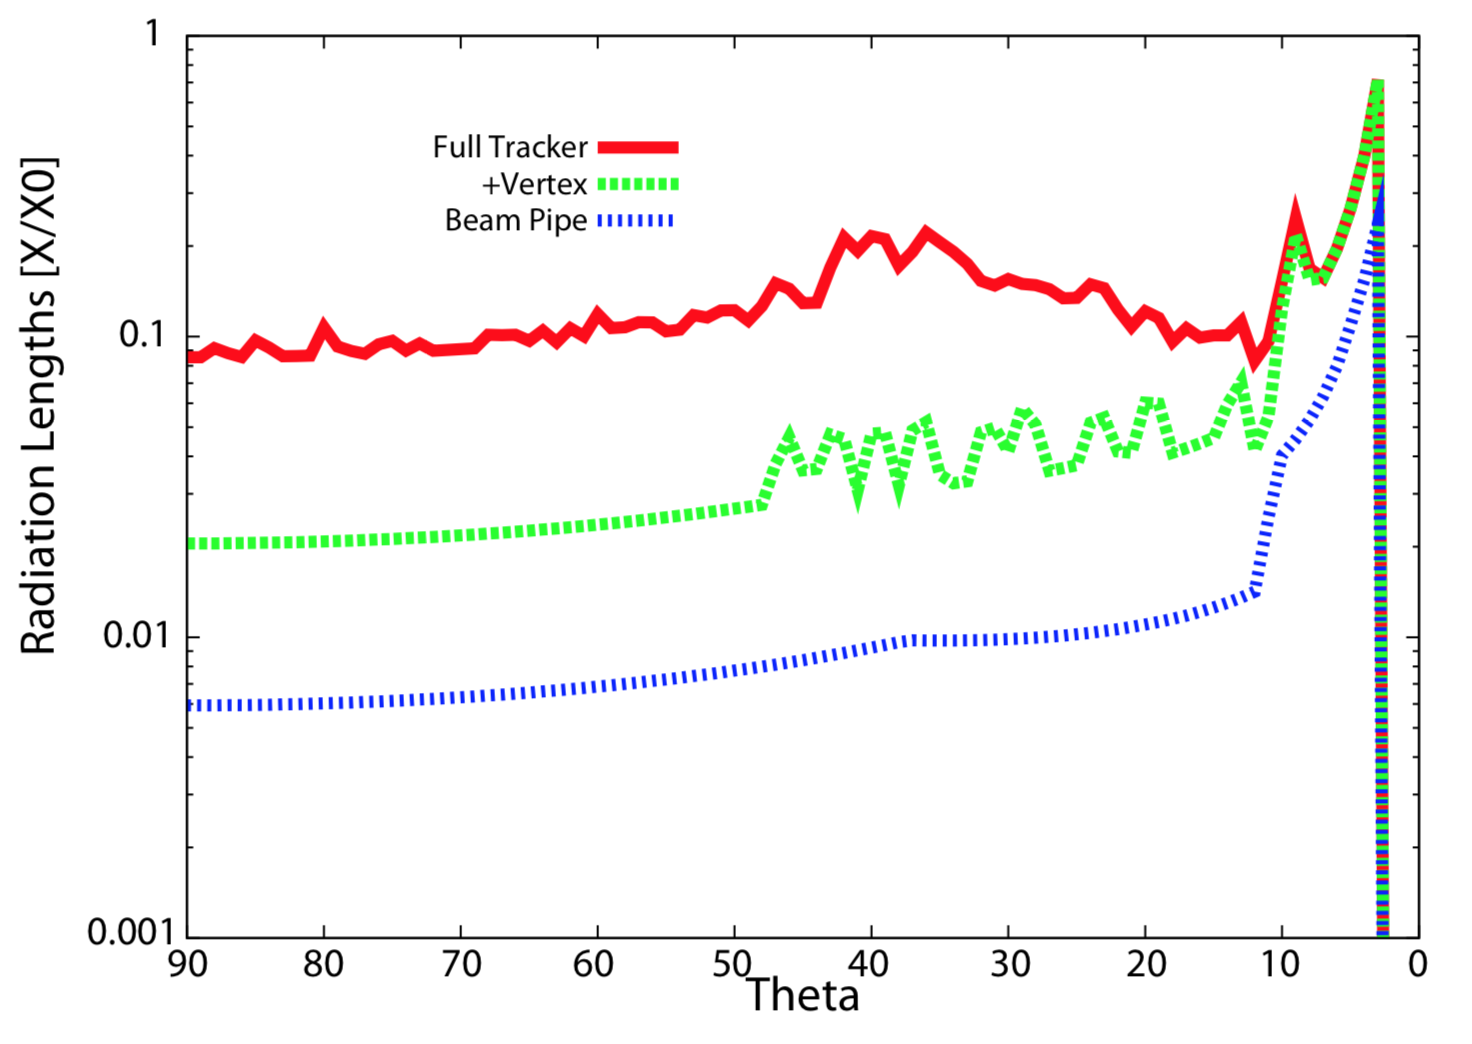
\includegraphics[width=0.80\hsize]{./chapters/figures/SiD_material_budget_tracker.png}
\end{center}
\caption{Material in the SiD detector, in terms of fractions of a radiation length, as a function of the polar angle.}
\label{fig:sid_mat_budget}
\end{figure}
%%%%%%%%%%%%%%%%%


The all-silicon tracking approach has been extensively tested using full Monte-Carlo
simulations including full beam backgrounds. Besides having an excellent momentum resolution
it provides robust pattern recognition even in the presence of backgrounds and has a
real safety margin, if the machine backgrounds will be worse than expected.

\subsubsection{Main calorimeters}

The SiD  baseline design incorporates the elements needed to
successfully implement the PFA approach. This imposes a number of
basic requirements on the calorimetry. The central calorimeter
system must be contained within the solenoid in order to reliably associate
tracks to energy deposits. The electromagnetic and hadronic sections
must have imaging capabilities that allow both efficient
track-following and correct assignment of energy clusters to tracks. These
requirements imply that the calorimeters must be finely segmented both
longitudinally and transversely. In order to ensure that no significant amount
of energy can escape detection, the calorimetry must extend down to small
angles with respect to the beampipe and must be sufficiently deep to prevent
significant energy leakage. Since the average penetration depth of a hadronic
shower grows with its energy, the calorimeter system must be designed for the
highest-energy collisions envisaged.

In order to ease detector construction the calorimeter mechanical design consists of a series of modules of
manageable size and weight. The boundaries between
modules are kept as small as possible to prevent significant non-instrumented
regions. The detectors are designed to have excellent long-term stability and reliability,
since access during the data-taking period will be extremely limited, if not
impossible.

The combined ECAL and HCAL systems consist of a
central barrel part and two endcaps, nested inside the barrel. The entire barrel system is contained
within the volume of the cylindrical superconducting solenoid. 

%The
%electromagnetic calorimeter has silicon active layers between tungsten absorber
%layers. The active layers use 5$\times$5~mm$^2$ silicon pixels, which provide excellent spatial resolution.
%The structure has 30 layers in total, the first 20 layers having a
%thinner absorber than the last ten layers. This configuration is a 
%compromise between cost, electromagnetic shower radius, sampling frequency, and
%shower containment. The total depth of the electromagnetic calorimeter is 26
%radiation lengths (\xo) and one nuclear interaction length. 

SiD's reliance on particle flow calorimetry to obtain a jet energy resolution of  $\sim$3\% demands a highly segmented (longitudinally and laterally) electromagnetic calorimeter. It also calls for a minimized lateral electromagnetic shower size, by minimizing the Moliere radius to efficiently separate photons, electrons and charged hadrons~\cite{calor:2018}.

The SiD ECal design employs thirty longitudinal layers, the first twenty each with 2.50 mm tungsten alloy thickness and 1.25 mm readout gaps, and the last ten with 5.00 mm tungsten alloy.  The total depth is 26 radiation lengths, providing good containment of electromagnetic showers.

Simulations have shown the energy resolution for electrons or photons
to be well described by 0.17 / $\sqrt{E}$ $\oplus$ 0.009, degrading a
bit  at higher energies due to changes in sampling fraction and a small leakage.

The baseline design employs tiled, large, commercially produced silicon sensors (currently assuming 15 cm wafers). The sensors are segmented into pixels that are individually read out over the full range of charge depositions. The complete electronics for the pixels is contained in a single chip, the KPiX ASIC~\cite{Brau:2013yb}, which is bump bonded to the wafer. The low beam-crossing duty cycle ($10^{-3}$) allows reducing the heat load using power pulsing, thus allowing passive thermal management within the ECal modules.

Bench tests of the KPiX bonded sensor  with a cosmic ray telescope trigger yielded 
a Landau distribution with a peak of the signal at about 4 fC is consistent with our expectation for minimum-ionizing particles (MIP) passing through the fully-depleted 320 $\mu$m thick sensors. Crosstalk between channels has been managed and the 
 noise distribution shows an RMS of 0.2 fC, well below the 4 fC MIP signal, and exceeding the ECal requirement.

The overall mechanical structure of the ECal barrel has been designed for minimal uninstrumented gaps. Input power and signals are delivered with Kapton flex cables.
The KPiX chip has an average power less than 20 mW, resulting in a
total heat load  that is managed with a cold plate and water pipes routed 
into the calorimeter.

A first SiD ECal prototype stack of nine (of thirty) layers has been constructed and was exposed to a 12.1 GeV electron beam at the SLAC End Station Test Beam Facility. 
This data collection demonstrated good measurements of multiple particle overlap and reconstruction of overlapping showers~\cite{Steinhebel:2017qze}.  Comparison of the deposited energy distribution in each of the nine layers also agrees well with simulations.
An algorithm developed to count the number of incident electrons in each event. The algorithm was used to assess the ability of the calorimeter to separate two showers as a function of the separation of the showers, achieving 100\% for separations of $>$10 mm.



The hadronic
calorimeter has a depth of 4.5 nuclear interaction lengths, consisting of
alternating steel plates and active layers. The baseline choice for the active
layers is scintillator tiles read out via silicon photomultipliers. For this approach SiD is closely following the analog hadron calorimeter developments within the CALICE collaboration. In this context, the simulated HCAL energy resolution has been shown to reproduce well the results from the CALICE AHCAL prototype module exposed to pion beams.

\subsubsection{Forward calorimeters}
\label{susub:det:forward}
Two special calorimeters are foreseen in the very forward region: LumiCal for a precise luminosity measurement, and BeamCal for the fast estimation of the collision parameters and tagging of forward-scattered beam particles. LumiCal and BeamCal are both compact cylindrical electromagnetic calorimeters centered on the outgoing beam, making use of semiconductor-tungsten technology. BeamCal is placed just in front of the final focus quadrupole and LumiCal is aligned with the electromagnetic calorimeter endcap. 

LumiCal makes use of conventional silicon diode sensor readout. It is a precision device with challenging requirements on the mechanics and position control, and must achieve a small Moliere radius to reach its precision targets. Substantial work has been done to thin the silicon sensor readout planes within the silicon-tungsten assembly. Dedicated electronics with an appropriately large dynamic range is under development.

BeamCal is exposed to a large flux of low-energy electron-positron pairs originating from beamstrahlung. These depositions, useful for a bunch-by-bunch luminosity estimate and the determination of beam parameters, require radiation hard sensors. The BeamCal has to cope with 100\% occupancies, requiring dedicated front-end electronics. A challenge for BeamCal is to identify sensors that will tolerate over one MGy of ionizing radiation per year. Sensor technologies under consideration include polycrystalline chemical vapor deposition (CVD) diamond (too expensive to be used for the full coverage), GaAs, SiC, Sapphire, and conventional silicon diode sensors. The radiation tolerance of all of these sensor technologies has been studied in a high-intensity electron beam. 

For SiD, the main activities are the study of these radiation-hard sensors, development of the first version of the so-called Bean readout chip, and the simulation of BeamCal tagging for physics studies. SiD coordinates these activities through its participation in the FCAL R\&D Collaboration.

\subsubsection{Magnet Coil}

The SiD superconducting solenoid is based on the CMS solenoid
design philosophy and construction techniques, using a slightly modified CMS
conductor as its baseline design. Superconducting strand count in the coextruded
Rutherford cable was increased from 32 to 40 to accommodate the higher 5~T
central field. 

Many iron flux return configurations have been simulated in two
dimensions so as to reduce the fringe field. An Opera 3D calculation with the Detector
Integrated Dipole (DID) coil has been completed.
Calculations of magnetic field with a 3D ANSYS program
are in progress. These will have the capability to calculate forces and stress
on the DID as well as run transient cases to check the viability of using the
DID as a quench propagator for the solenoid. Field and force calculations with
an iron endcap HCAL were studied. The field homogeneity improvement was found
to be insufficient to pursue this option. 

Conceptual DID construction and
assembly methods have been studied. The solenoid electrical power system,
including a water-cooled dump resistor and grounding, was established.
Significant work has been expended on examining different conductor stabiliser
options and conductor fabrication methods. This work is pursued as a cost- and
time-saving effort for solenoid construction.

\subsubsection{Muon System}
The flux-return yoke is instrumented with position sensitive detectors to
serve as both a muon filter and a tail catcher. The total area to be
instrumented is very significant -- several thousand square meters. Technologies
that lend themselves to low-cost large-area detectors are therefore under
investigation. Particles arriving at the muon system have seen large amounts of
material in the calorimeters and encounter significant multiple scattering
inside the iron. Spatial resolution of a few centimetres is therefore
sufficient. Occupancies are low, so strip detectors are possible. The SiD 
baseline design uses scintillator technology, with RPCs as an alternative. 
The scintillator technology uses extruded scintillator readout with wavelength 
shifting fibre and SiPMs, and has been successfully demonstrated. 
Simulation studies have shown that nine or more layers of sensitive detectors 
yield adequate energy measurements and good muon-detection efficiency and purity.
The flux-return yoke itself has been optimised with respect to the
uniformity of the central solenoidal field, the external fringe field,
and ease of the iron assembly. 
This was achieved by separating the  barrel and end sections of the
yoke along a 30 degree line.

\subsubsection{The Machine-Detector Interface}
A time-efficient implementation of the push-pull model of
operation sets specific requirements and challenges for many detector and
machine systems, in particular the interaction region (IR) magnets, the
cryogenics, the alignment system, the beamline shielding, the detector design
and the overall integration. The minimal functional requirements and interface
specifications for the push-pull IR have been successfully developed and
published~\cite{Platform_Agreement,IR_Layout}.  All further IR design
work on both the detectors and machine sides are constrained by these 
specifications. 

\subsection{The ILD Detector}
The ILD detector is a proposed detector for the ILC. It has been developed by a proto-collaboration with the goal to develop and eventually propose a fully integrated detector for the ILC. 

The ILD detector concept has been designed as a multi-purpose detector. It should deliver excellent physics performance for collision energies between 90~Gev and 1~TeV, the largest possible energy reach of the ILC. The ILD detector has been optimized to perform excellently at the initial ILC energy of 250 GeV (for more details see \cite{ild:bib:ILDloi,ild:bib:ILDDBD}). An artists view of the ILD detector is shown in Fig.~\ref{fig:ild_3d}. 
\begin{figure}
    \centering
    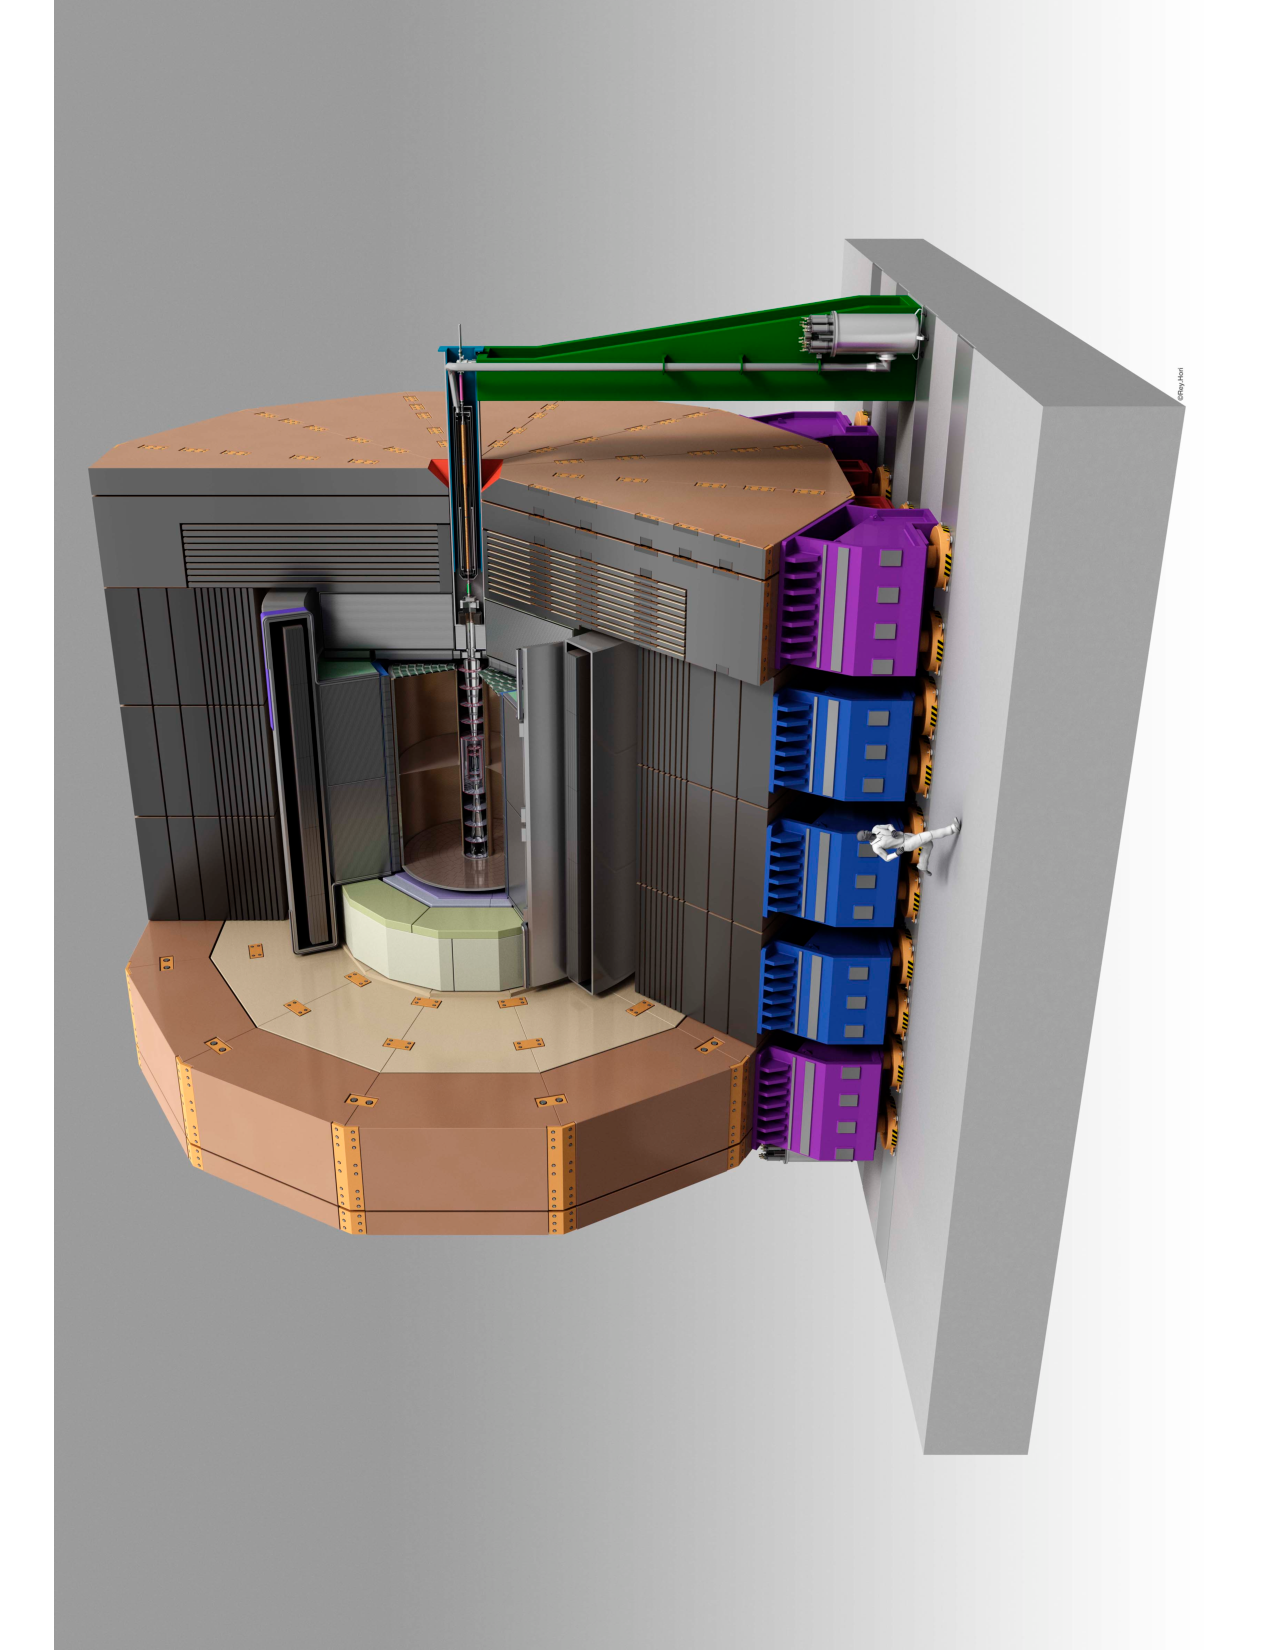
\includegraphics[width=0.35\textwidth]{../figures/ILD.pdf}
    \caption{3D-picture of the ILD detector.}
    \label{fig:ild_3d}
\end{figure}

The science which will be done at the ILC requires a detector that
truly covers all aspects of the $\ee$ events.  The tracking philosophy
is very different from that of SiD, as will be discussed in a moment.
However, similarly to SiD, the ILD detector has been designed to combine the traditional
precision detector 
elements such as as vertex detectors and trackers in an overall design
philosophy 
that optimizes jet reconstruction using particle flow. 


\subsubsection{Vertexing and Tracking}
\label{subsubsec:ILDtracker}
The high precision vertex detector positioned very closely to the
interaction point is followed by a hybrid tracking layout, realised as
a combination of silicon tracking with a time projection chamber, and
a calorimeter system. The complete system is located inside a large
solenoid providing a magnetic field of 3.5-4 T. On the outside of the
coil, 
the iron return yoke is instrumented as a muon system and as a tail catcher calorimeter. 

The vertex detector is realised as a multi-layer pixel-vertex detector
(VTX), with three super-layers, each comprising two layers. The
detector
 has a pure barrel geometry. To minimise the occupancy from background hits,
the first super-layer is only half as long as the outer two. Whilst the underlying detector technology has not yet been decided, 
the VTX is optimised for point resolution and
 minimum material thickness. 
	
A system of silicon strip and pixel detectors surrounds the VTX detector. In the barrel, two layers of silicon strip detectors (SIT) are arranged to bridge the gap between the VTX and the TPC. In the forward region, a system of two silicon-pixel disks and five silicon-strip disks (FTD) provides low angle tracking coverage.

A distinct feature of ILD is a large volume time projection chamber
(TPC) with up to 224 points per track. The TPC is optimised for
3-dimensional point resolution and minimum material in the field cage
and in the end-plate. It also allows d$E$/d$x$-based particle
identification. At the ILC,  a TPC has a number of specific strengths
 which make this type of detector attractive. A time projection
 chamber offers true three-dimensional points, and offers many of
 those along a charged particle trajectory. The intrinsic disadvantage
 of a TPC, its slow readout speed, does not harm the
 performance at the ILC, since the time between bunches is relatively
 long, around 300~ns. On the other hand the large number of
 points offer superb pattern recognition capabilities, and allows the
 detailed reconstruction of kinks or decays in flight within its
 volume. This can be achieved at a very low material budget, rather
 uniformly distributed over the sensitive volume. The excellent
 performance of the system is particularly striking at low momenta, at
 a few GeV and below, where the combination of three dimensional
 reconstruction and low material 
allows the efficient and precise reconstruction of tracks. 

Outside the TPC, a system of Si-strip detectors in between the TPC and
the ECAL (SET), provide additional high precision space points which
 improve the tracking performance and provide additional
    redundancy in the regions between the main tracking volume and the
    calorimeters. 

A key aspect of the ILD detector design is the low mass of the tracking system. The total material as a function of angle, in radiation lengths, is shown in Fig.~\ref{fig:ILD_mat_budget}.

%%%%%%%%%%%%%%%%%%%%%%%%%%%%%%%%%%%%%%%%%%%%%%%%%%%%%
\begin{figure}
\centering
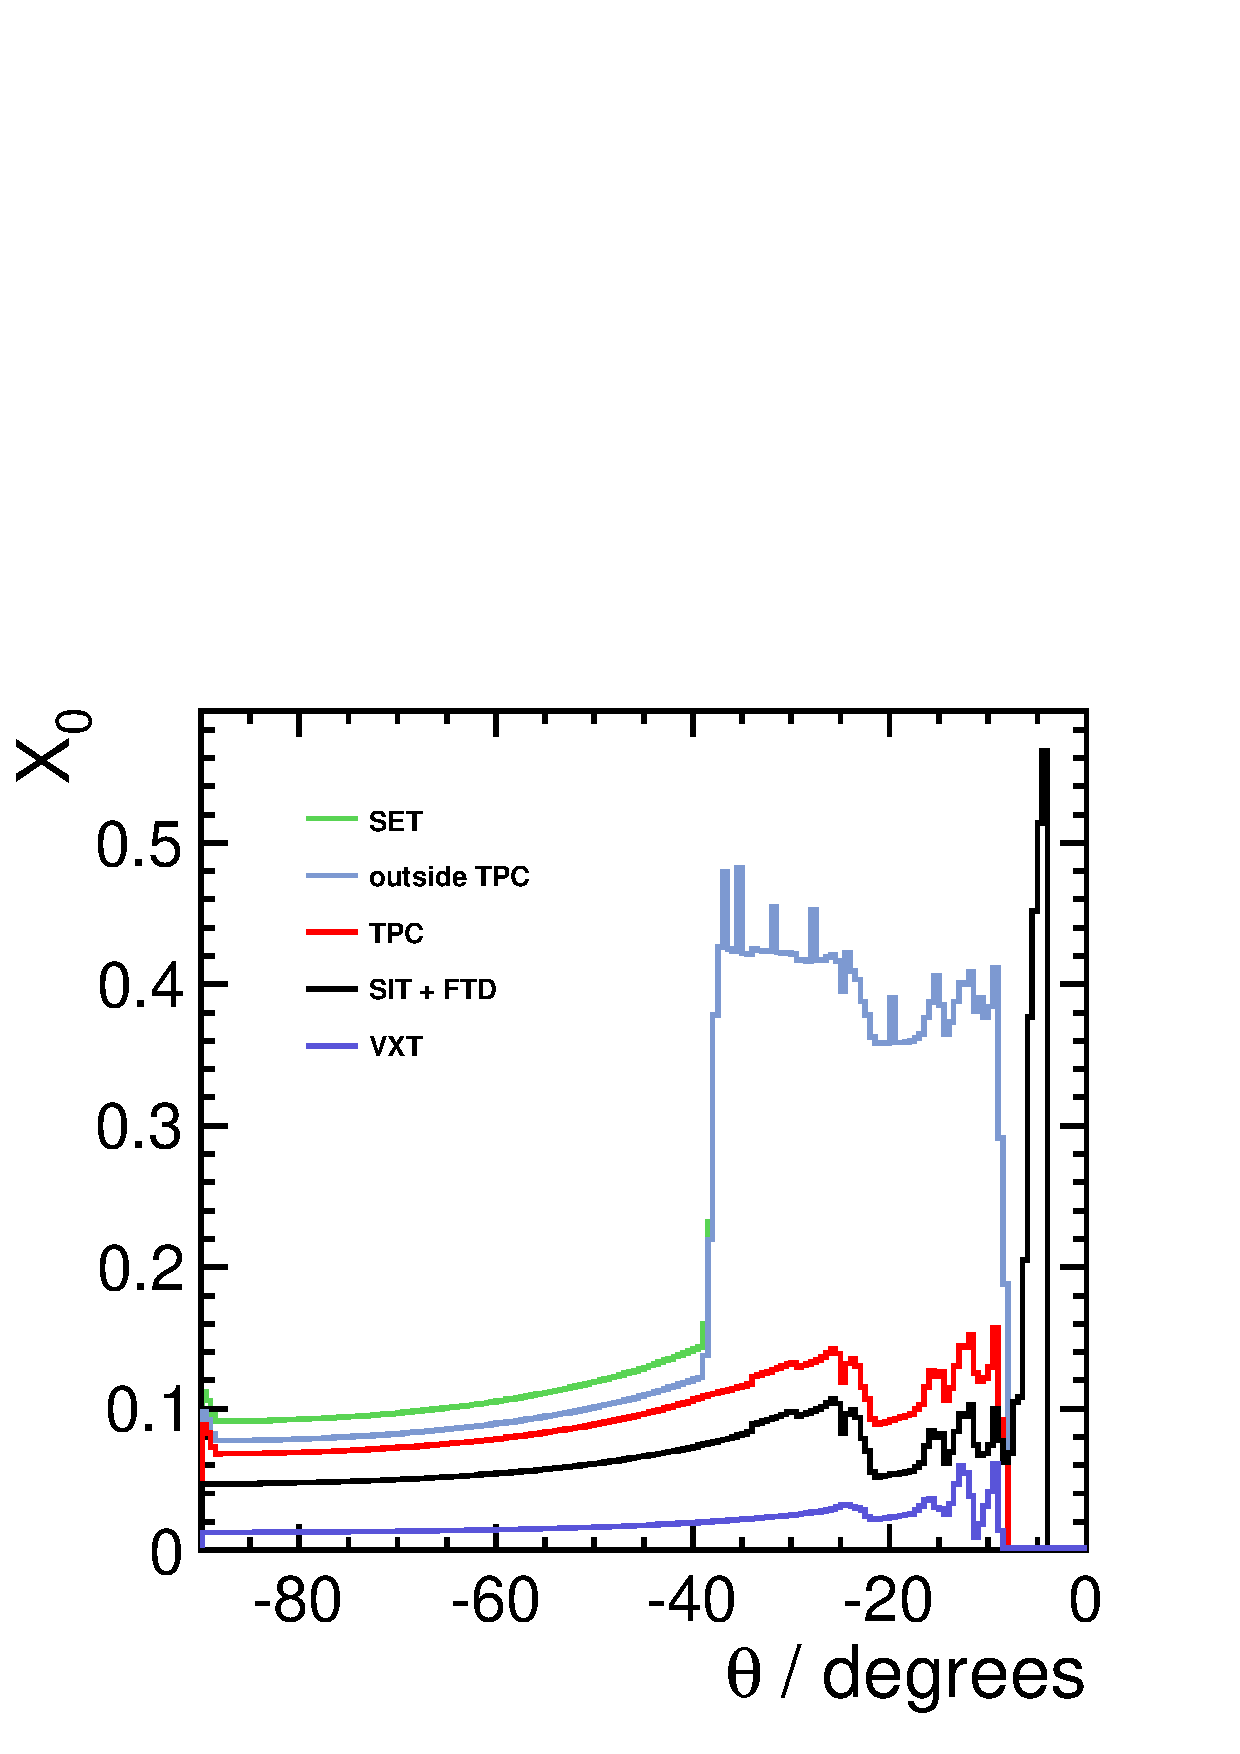
\includegraphics[width=0.85\hsize,viewport={0 -10 600 500},clip]{chapters/figures/material-budget-new.pdf}
\caption{Material in the ILD detector, in terms of fractions of a radiation length, as a function of the polar angle.}
\label{fig:ILD_mat_budget}
\end{figure}
%%%%%%%%%%%%%%%%%%%%%%%%%%%%%%%%%%%%%%%%%%%%%%%%%%%

\subsubsection{Calorimetry}

A highly segmented electromagnetic calorimeter (ECAL) provides up to
30 samples in depth and small transverse cell size, split into a
barrel and an end cap system. For the absorber, Tungsten has been
chosen; for the sensitive area, silicon diodes 
or scintillator strips are considered.

% %\thisfloatsetup{floatwidth=\SfigwFull,capposition=beside}
% \begin{figure}[t!]
% \begin{tabular}{cc}
% 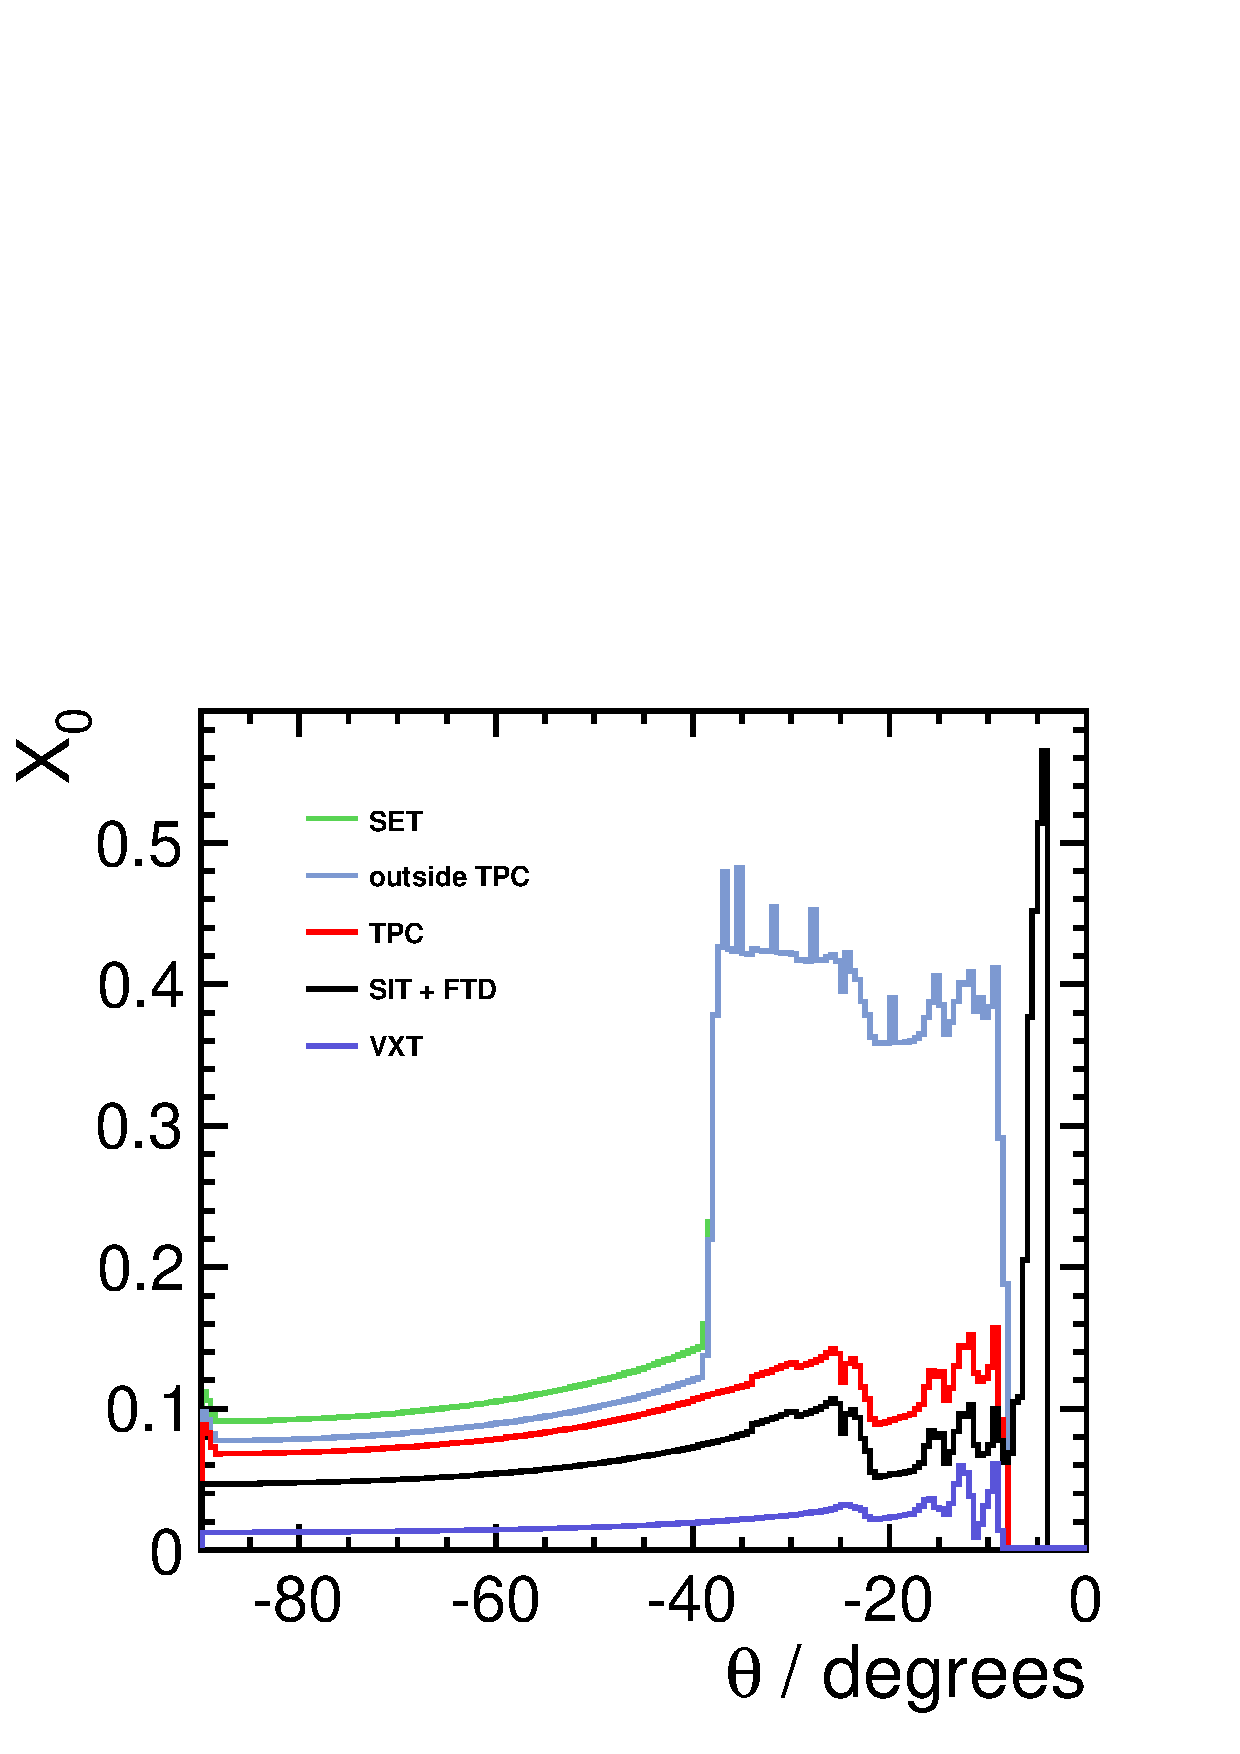
\includegraphics[width=0.52\hsize,viewport={0 -10 600 500},clip]{chapters/figures/material-budget-new.pdf} &
% 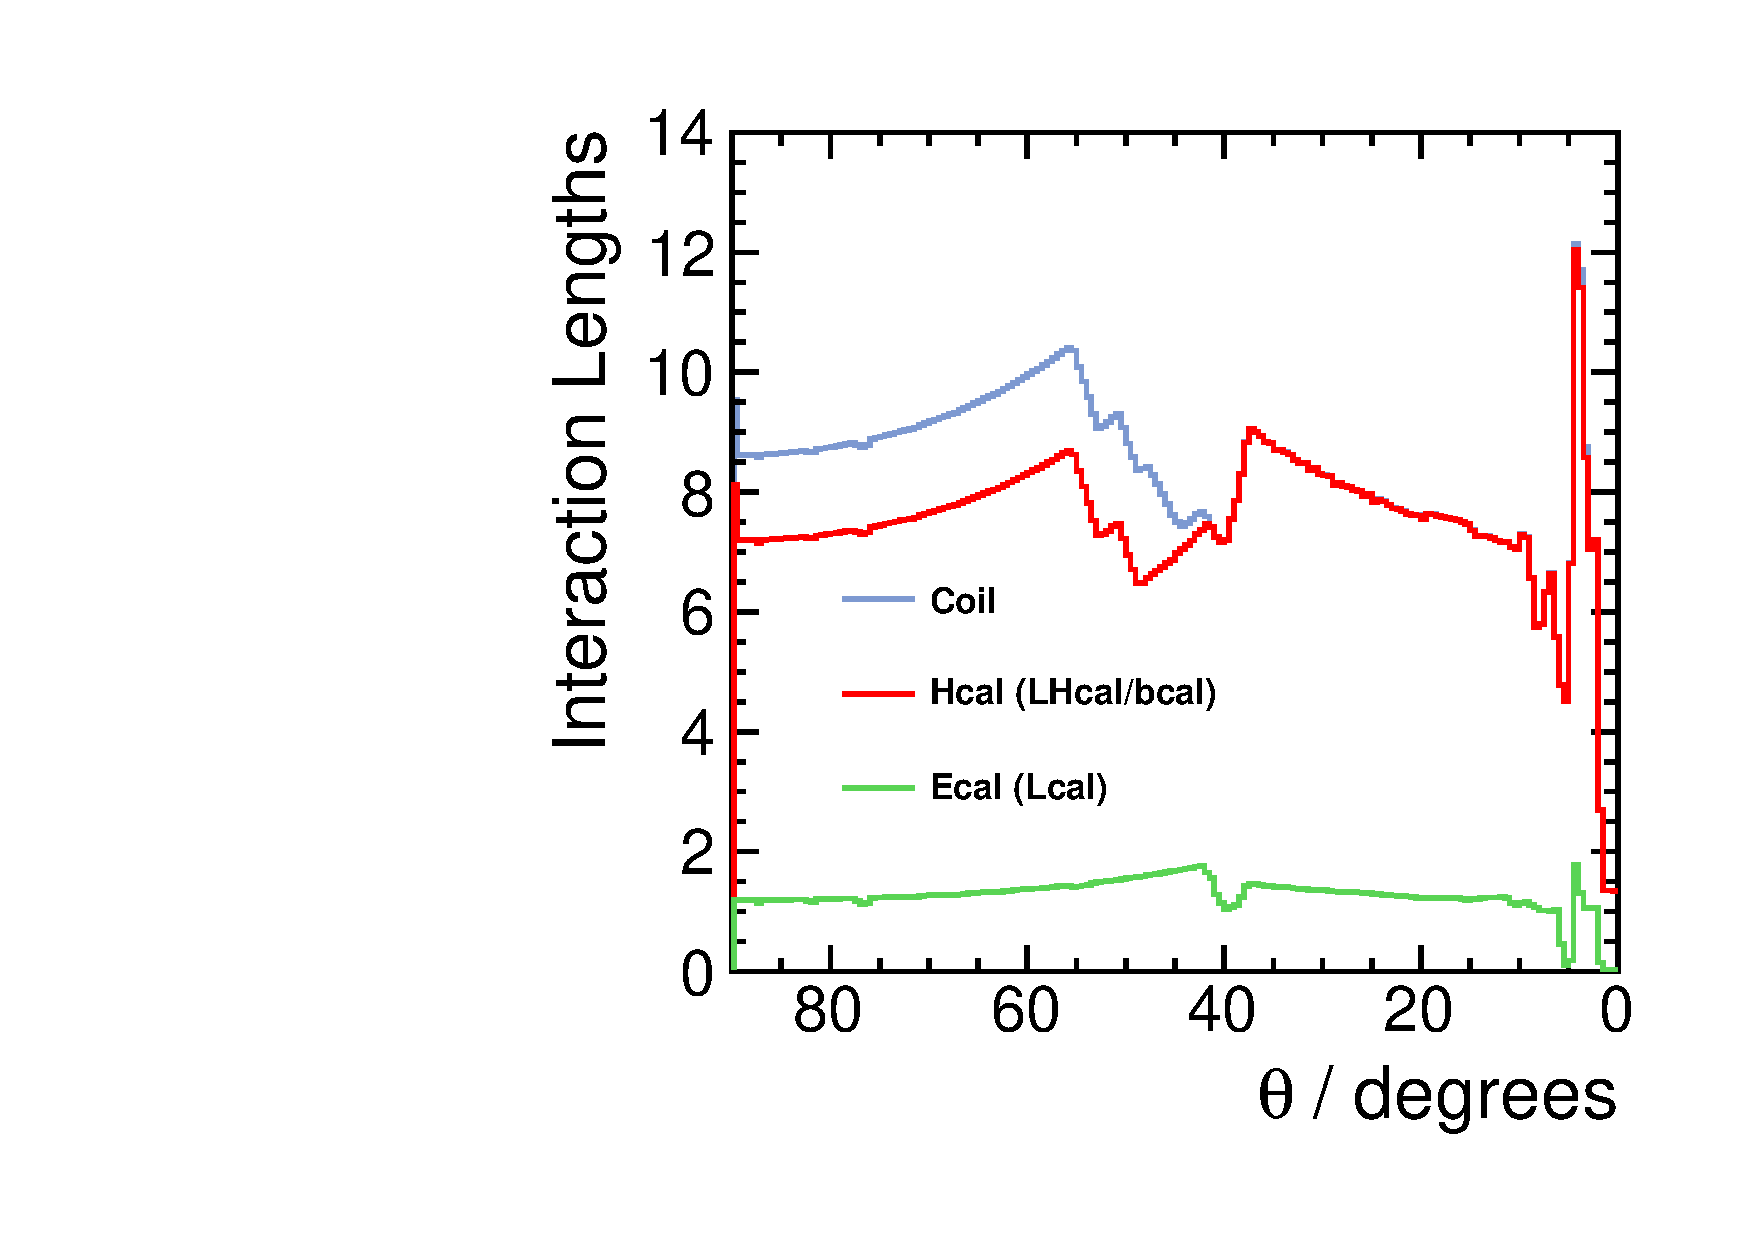
\includegraphics[width=0.5\hsize]{chapters/figures/intlen_ILD_o1_v05.pdf}
% \end{tabular}
% \caption[Material in the ILD detector]{Left: Average total radiation length of the material
%   in the tracking detectors as a function of polar angle. Right: Total
%   interaction
%  length in the detector, up to the end of the calorimeter system, and including the coil of the detector.}
% %\end{figure}
% \label{ild:fig:intro:material}
% %\begin{tabular}{cc}

% \end{figure}

This is followed by a segmented hadronic calorimeter (HCAL) with up to 48 longitudinal samples and small transverse cell size. Two 
options are considered, both based on a steel-absorber structure. One option uses scintillator tiles of $3 \times 3$\,cm$^2$, 
which are read out with an analogue system. The second uses a gas-based readout which allows a $1 \times 1$\,cm$^2$ 
cell geometry with a semi-digital readout of each cell. 

At very forward angles, below the coverage provided by the ECAL and
the HCAL, a system of high precision and radiation hard calorimetric
detectors (LumiCAL, BeamCAL, LHCAL)
 is foreseen. The LumiCAL and BeamCAL are based on technologies developed in the context of the FCAL collaboration. These detectors 
extend the calorimetric coverage to almost $4\pi$, measure the
luminosity, and  monitor
 the quality of the colliding beams. the LHCAL system bridges the electromagnetic endcap calorimeter with the forward systems. 

\subsubsection{Coil and Yoke}
A large volume superconducting coil surrounds the calorimeters, creating an axial $B$-field of nominally 3.5-4\,Tesla.

An iron  yoke, instrumented with scintillator strips or resistive
plate chambers (RPCs), returns the magnetic flux of the solenoid, and,
at the same
 time, serves as a muon filter, muon detector and tail catcher calorimeter.

\subsubsection{Detector Integration and Performance}
The ILD detector is designed to operate in the ILC interaction region with a push-pull scheme, allowing the rapid interchange of ILD with SiD. Detailed studies have been done to understand the impact this scheme might have on the detector and its design. In addition the ILD detector is optimised for operation in the seismic active region in the north of Japan. Extensive simulation studies for the main components have shown that the detector is stable against seismic events. 

% %\thisfloatsetup{floatwidth=\SfigwFull,capposition=beside}
% \begin{figure}[b!]
% \begin{tabular}{cc}

% 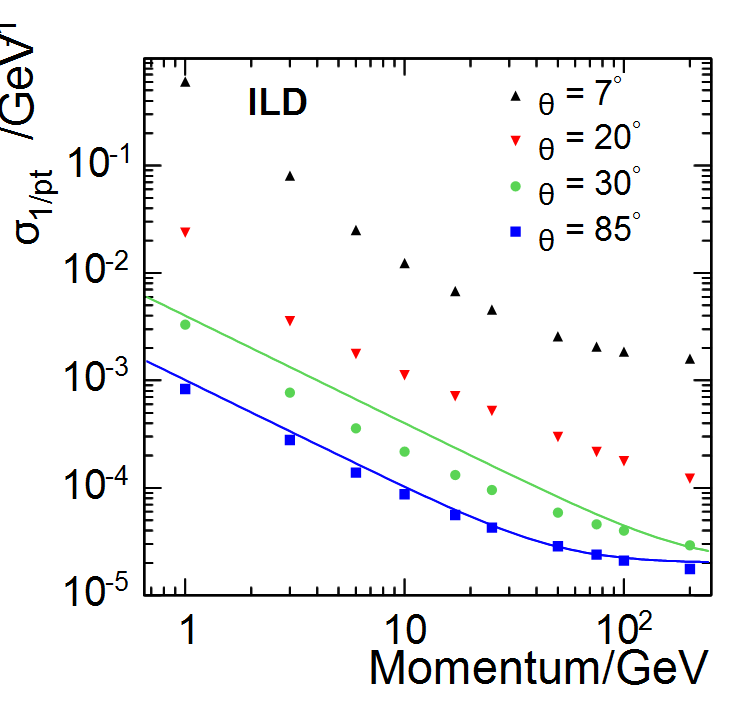
\includegraphics[width=0.5\hsize]{chapters/figures/deltaInvP_all_fits.png} &
% 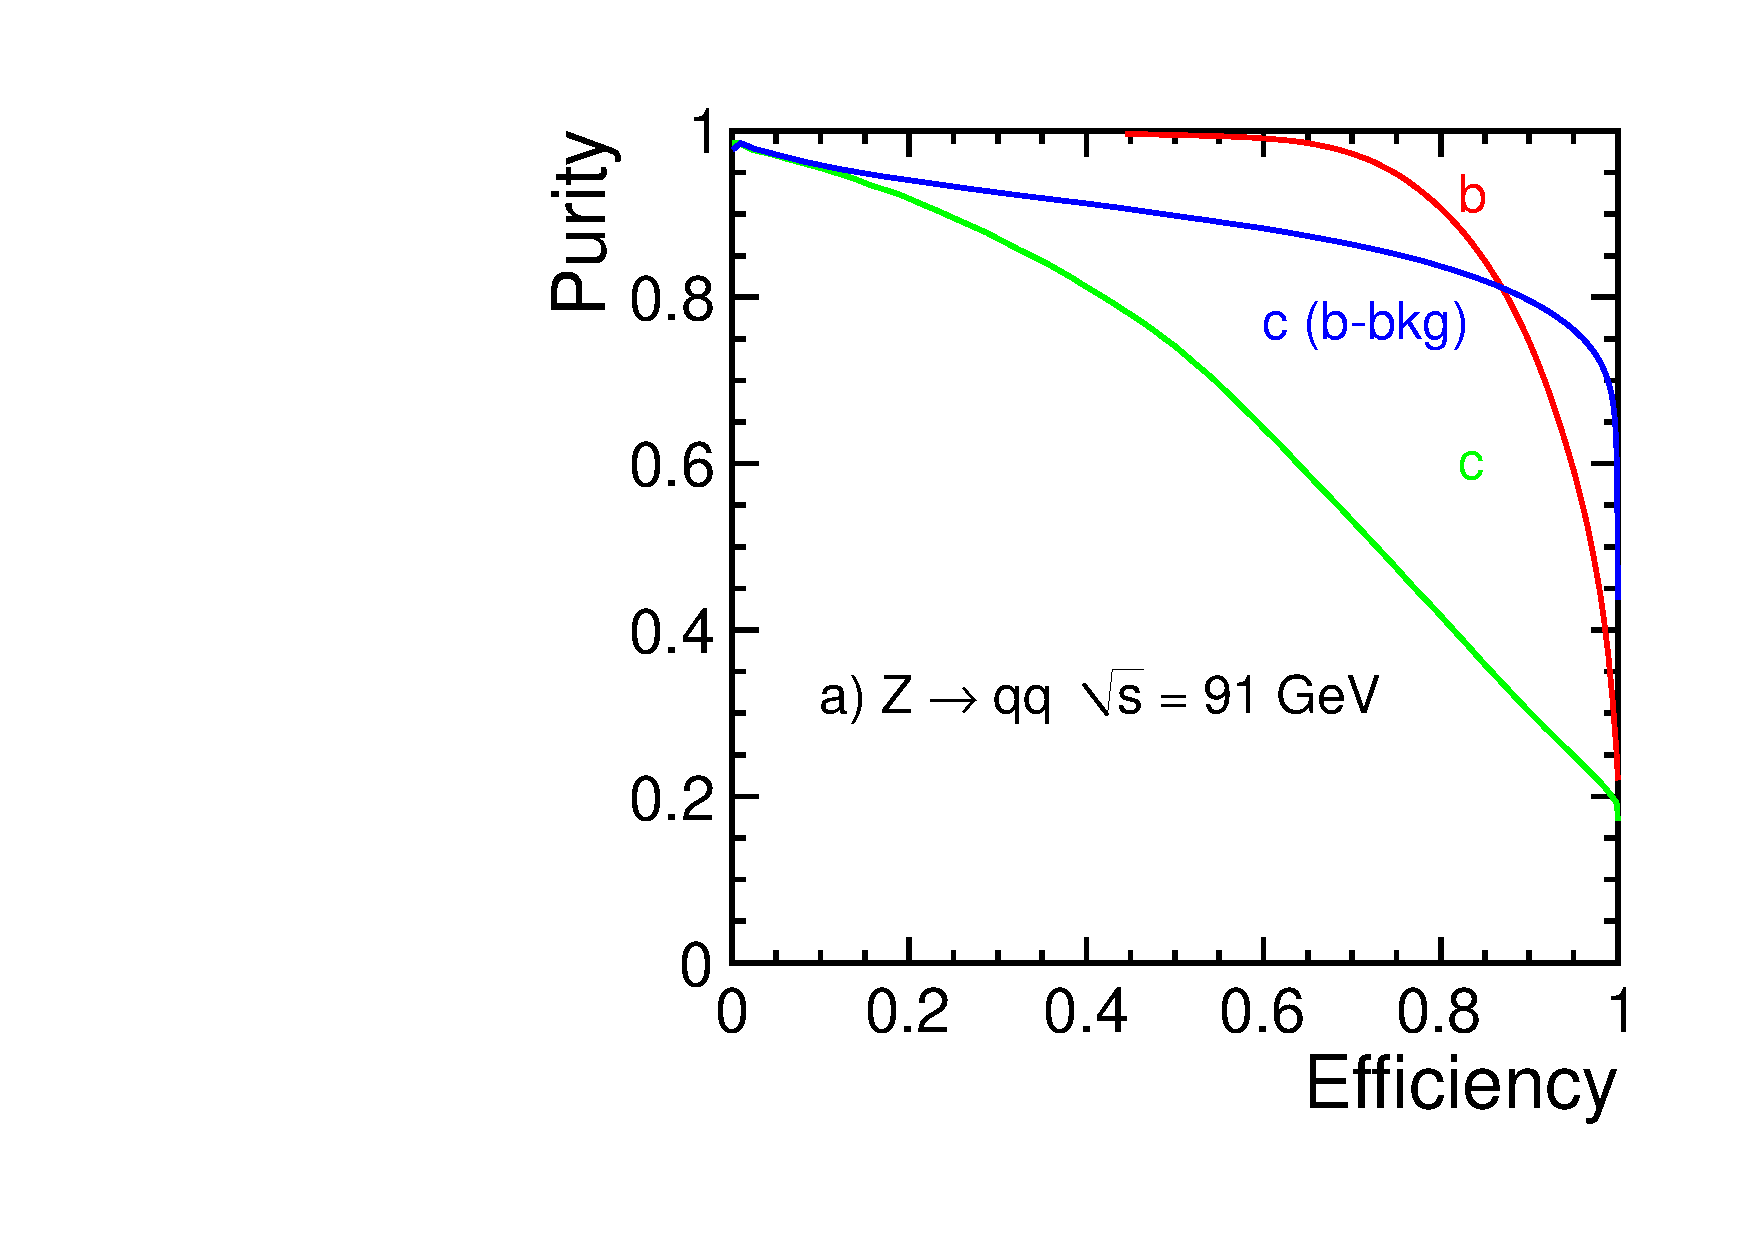
\includegraphics[width=0.5\hsize]{chapters/figures/evalZ-lcfiweights_qq91new_v02-test.pdf}
% \end{tabular}
% \caption{\label{ild:fig:intro:tracking}(left) Momentum resolution for the ILD detector concept, as a function of the transverse momentum of the particle. (right) Flavour tagging efficiency versus purity for bottom events in sample of Z decays at 91\,GeV, and for charm events with only bottom background. )}
% \end{figure}



% \begin{figure}[t!]

% 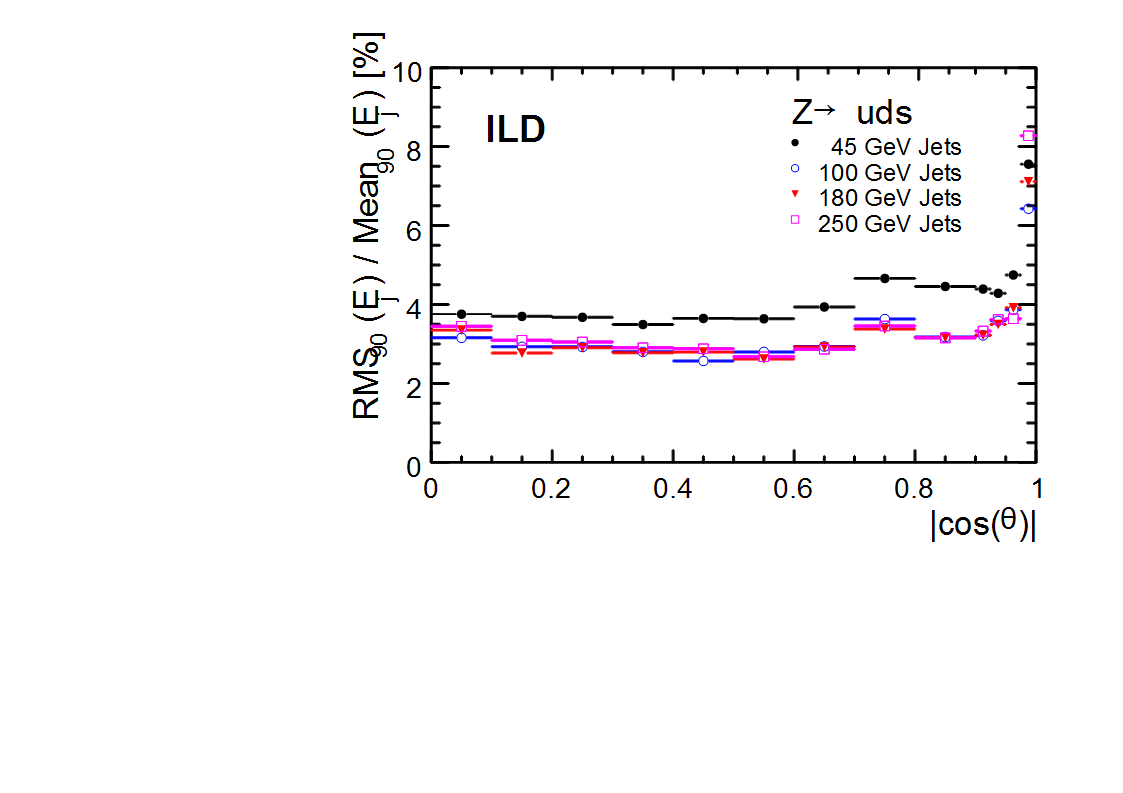
\includegraphics[width=0.8\hsize]{chapters/figures/ild01_o1_pflow.png}

% \caption{\label{ild:fig:intro:pflow}Fractional jet energy resolution
%     plotted against $|\cos\theta|$ where theta is the polar angle of the thrust axis of the event. }
% \end{figure}

% %The main parameters of the ILD detector are summarised in Table~\ref{ild:tab:barrelpara} and table~\ref{ild:tab:endcappara}.
% %\begin{sidewaystable}[thb]

% \subsubsection{ILD Performance}
% The performance of the ILD concept has been extensively studied using a detailed GEANT4 based simulation model and sophisticated reconstruction tools. Backgrounds have been taken into account to the best of current knowledge. 

% The key technologies proposed for the ILD detector have been developed in close cooperation with R\&D collaborations and have been extensively tested. The performance numbers of key systems are based on results from prototypes, whereever possible, and extraploated to the full detector performance. This strong check against experimental results ensures that the performance numbers are reliable and are considered a realistic estimate of the ultimate detector performance. 


% A key characteristics of the detector is the amount of material in the detector. Particle flow requires a thin tracker, to minimise interactions before the calorimeters, and thick calorimeters, to fully absorb the showers. Figure~\ref{ild:fig:intro:material}~(left) shows the material in the detector in radiation lengths, until the entry of the calorimeter. The right plot shows the total interaction length including the calorimeter system. 

% The performance of the tracking system can be summarised by its combined momentum resolution, shown in Figure~\ref{ild:fig:intro:tracking}~(left). A resolution of $\sigma_{1/p_T} = 2 \times 10^{-5}$\,GeV$^{-1}$ has been achieved for high momenta. For many physics studies the tagging of long lived particles is of key importance. Several layers of pixel detectors close to the IP allow the reconstruction of displaced vertices, as shown in Figure~\ref{ild:fig:intro:tracking}~(right).

% Calorimeter system and tracking system together enter into the particle flow performance. The performance of the ILD detector for different energies and as a function of the polar angle is shown in Figure~\ref{ild:fig:intro:pflow}. 

% The few plots shown in this section illustrate the anticipated performance of the detector and illustrate the potential for precision measurements with the ILD detector. 

Key plots to evaluate the projected performances of the ILD and SiD
detectors will be presented in the following chapter.    These plots
will also illustrate the successive stages of event reconstruction
from raw data and will describe the level of detail that we have
considered in making these estimates of performance.  
As we have already noted, the ILD and SiD detectors include many
technologies that have been developed in close cooperation with R\&D
collaborations 
and have been extensively tested. For both detectors, the performance numbers 
of key systems are based on results from prototypes, wherever 
possible, and extrapolated to the full detector performance. This
strong 
check against experimental results ensures that the performance 
numbers are reliable and are considered a realistic estimate of the ultimate detector performance. 
